\documentclass[12pt,twoside]{article}

\setlength{\textwidth}{166mm}
\setlength{\textheight}{232mm}
\setlength{\topmargin}{-10mm}
\setlength{\headsep}{5mm}
\oddsidemargin=3mm
\evensidemargin=3mm
\setlength{\baselineskip}{18pt}

\usepackage[utf8]{inputenc}
\usepackage[russian]{babel}
\usepackage{amsfonts,amssymb,amsmath}
\usepackage{epsfig}
\usepackage{mathrsfs}
\usepackage{mathabx}
\usepackage{xcolor}

\renewcommand\le{\leqslant}
\renewcommand\ge{\geqslant}

\newcommand{\ruText}[1]{
  {\footnotesize \textcolor{darkgray}{#1} \par}
}

\newcommand{\biLangHeader}[2]{
  \subsection*{%
  	#1 \\%
  	\ruText{#2}%
  }%
}

\newcommand{\quizTitle}[3]{%
\begin{center}
	\textbf{Кантрольная работа па тэме <<#1>> (варыянт #3)} \\
	\ruText{Контрольная работа по теме <<#2>> (вариант #3)}
\end{center}
}

\newcommand{\problemItemSimple}[2]{%
	\item #1 \\%
	\ruText{#2}%
}

\newcommand{\problemItemWithCommonPart}[3]{%
	\item #1 \\%
	\ruText{#2}%
	#3%
}

\newcommand{\problemItemWithCommonPartComplicated}[5]{%
	\item #1 \\%
	\ruText{#2}%
	#3 \\
	\noindent #4 \\%
	\noindent \ruText{#5}%
}

\makeatletter
\def\belarusianLetters#1{
  \expandafter\@belarusianLetters\csname c@#1\endcsname
}
\def\@belarusianLetters#1{
  (%
  \ifcase#1\or а\or б\or в\or г\or д\or е\or ж\or з\or і\or к\or л\or м\fi%
  )
}
\makeatother
\AddEnumerateCounter{\belarusianLetters}{\@belarusianLetters}{Ы}

\newenvironment{problemList}
  {\begin{enumerate}[leftmargin=*,topsep=0pt,itemsep=-1ex,partopsep=1ex,parsep=1ex]}
  {\end{enumerate}}

\newenvironment{belarusianEnumerate}
  {\begin{enumerate}[label=\belarusianLetters*, topsep=-7pt]}
  {\end{enumerate} \textbf{}\vspace{-8pt}}

\AddEnumerateCounter{\asbuk}{\@asbuk}{\cyrm}
\newenvironment{russianEnumerate}
  {\begin{enumerate}[label=(\asbuk*), topsep=-4pt, itemsep=-1ex]}
  {\end{enumerate} \textbf{}\vspace{-11pt}}


% Lines below are to avoid word breaks.
\tolerance=1
\emergencystretch=\maxdimen
\hyphenpenalty=10000
\hbadness=10000

\renewenvironment{itemize}
{\begin{list}
             {\labelitemi}%                     Old parameters:
             {\setlength{\labelwidth}{1.3em}%        1em
              \setlength{\labelsep}{0.7em}%          0.7em
              \setlength{\itemindent}{0em}%          0em
              \setlength{\listparindent}{3em}%       3em
              \setlength{\leftmargin}{2em}%          3em !
              \setlength{\rightmargin}{0em}%         0em
              \setlength{\parsep}{0ex}%              0ex
              \setlength{\topsep}{0.5ex}%            2ex !
              \setlength{\itemsep}{1ex}%             0ex
             }
}
{\end{list}}

\pagestyle{empty}


\begin{document}
	\biLangHeader{3. Прыкладанні логікі выказванняў.}
	{Приложения логики высказываний.}
	
	\begin{problemList}
		\item Карыстаючыся законамі логікі выказванняў, дакажыце, што наступныя састаўныя выказванні праўдзівыя: \\
		\ruText{Пользуясь законами логики высказываний, докажите, что следующие составные высказывания истинны:}
		
		\begin{belarusianEnumerate}
			\item Рэчаісны лік $a > 2$ або $a < -1$ тады і толькі тады, калі з таго, што $a \le 2$, вынікае, што $a < -1$.\\
			\ruText{Действительное число $a > 2$ или $a < -1$ в том и только в том случае, когда из того, что $a \le 2$, следует, что $a < -1$.}
			
			\item Калі справядліва сцверджанне, што кожнае алгебраічнае раўнанне няцотнай ступені з рэчаіснымі каэфіцыентамі мае прынамсі адзін рэчаісны корань, то справядліва і сцверджанне, што кожнае алгебраічнае раўнанне з рэчаіснымі каэфіцыентамі, якое не мае рэчаіснага кораня, мае цотную ступень. \\
			\ruText{Если справедливо утверждение, что каждое алгебраическое уравнение нечетной степени с действительными коэффициентами имеет по меньшей мере один действительный корень, то справедливо и утверждение, что каждое алгебраическое уравнение с действительными коэффициентами, не имеющее действительного корня, имеет четную степень.}
		
			\item Два сцверджанні <<Сістэма $n$ лінейных аднародных раўнанняў з $n$ невядомымі мае адзінае рашэнне тады і толькі тады, калі вызначнік сістэмы не роўны нулю>>, і <<Сістэма $n$ лінейных аднародных раўнанняў з $n$ невядомымі мае прынамсі два рашэні тады і толькі тады, калі вызначнік сістэмы роўны нулю>>, адначасова праўдзівы або непраўдзівы. \\ 
			\ruText{Два утверждения: <<Система $n$ линейных однородных уравнений с $n$ неизвестными имеет единственное решение тогда и только тогда, когда определитель системы отличен от нуля>>, и <<Система $n$ линейных однородных уравнений с $n$ неизвестными имеет по меньшей мере два решения тогда и только тогда, когда определитель системы равен нулю>>, одновременно истинны или ложны.}
			
			\item Калі дыферэнцавальная функцыя непарыўная, то немажліва, каб функцыя была дыферэнцавальная і разрыўная. \\
			\ruText{Если дифференцируемая функция непрерывна, то невозможно, чтобы функция была дифференцируема и разрывна.}
			
			\item Калі справядліва, што нявыраджаная матрыца мае адваротную, то таксама справядліва, што матрыца выраджаецца ці мае адваротную. \\
			\ruText{Если справедливо, что невырожденная матрица имеет обратную, то справедливо также, что матрица вырождается или имеет обратную.}
		\end{belarusianEnumerate}
		
		\bigskip
		
		\item Калі заўтра студэнт пойдзе на першы занятак~$(A)$, то ён павінен будзе рана ўзняцца~$(B)$, а калі пойдзе ўвечары на дыскатэку~$(C)$, то ляжа спаць позна~$(D)$. Калі студэнт ляжа спаць позна і ўздымецца рана, то ён будзе вымушаны здавольвацца чатырма гадзінамі сну~$(E)$. Студэнт не здавольваецца чатырма гадзінамі сну. Ці вынікае адсюль, што студэнт павінны альбо прапусціць заўтра занятак, альбо не ісці ўвечары на дыскатэку? \\
		\ruText{Если завтра студент пойдет на первое занятие~$(A)$, то он должен будет рано встать~$(B)$, а если пойдет вечером на дискотеку~$(C)$, то ляжет спать поздно~$(D)$. Если студент ляжет спать поздно и встанет рано, то он будет вынужден довольствоваться четырьмя часами сна~$(E)$. Студент не обходится четырьмя часами сна. Следует ли отсюда, что студент должен или пропустить завтра занятие, или не ходить вечером на дискотеку?}
		
		\bigskip
		
		\item Калі будзе халодна~$(A)$, то студэнт апране цёплую куртку~$(B)$, калі рукаў будзе палатаны~$(C)$. Заўтра будзе халодна, а рукаў не будзе палатаны. Ці вынікае адсюль, што студэнт не апране цёплую куртку? \\
		\ruText{Если будет холодно~$(A)$, то студент наденет теплую куртку~$(B)$, если рукав будет починен~$(C)$. Завтра будет холодно, а рукав не будет починен. Следует ли отсюда, что студент не наденет теплую куртку?}
		
		\newpage
		
		\item Калі студэнт чытаў канспект на кухні, то акуляры ляжаць на кухонным стале. Калі акуляры ляжаць на кухонным стале, то студэнт бачыў іх за сняданкам. Ён не бачыў акуляры за сняданкам. Студэнт чытаў канспект у пакоі ці на кухні. Калі ён чытаў канспект у пакоі, то акуляры ляжаць на кафейным століку. Высветліце, дзе ляжаць акуляры? \\ 
		\ruText{Если студент читал конспект на кухне, то очки лежат на кухонном столе. Если очки лежат на кухонном столе, то студент видел их за завтраком. Он не видел очки за завтраком. Студент читал конспект в комнате или на кухне. Если он читал конспект в комнате, то очки лежат на кофейном столике. Выясните, где лежат очки?}
		
		\bigskip
		
		\item Чатыры спартоўцы "--- X, Y, Z і T "--- удзельнічалі ў спаборніцтве і занялі чатыры прызавыя месцы. Калі сталі дазнаваць, як размеркаваліся меcцы, атрымалі тры розныя адказы:
		\begin{belarusianEnumerate}
			\item Z першы, Y другі;			
			\item Z другі, T трэці;
			\item X другі, T чацвёрты.
		\end{belarusianEnumerate}
		У кожным адказе роўна адна частка з'яўляецца вернай. Пабудуйце мадэль для гэтай задачы ў тэрмінах формул логікі выказванняў і вызначыце правільнае размеркаванне месцаў. \\
		\ruText{Четыре спортсмена "--- X, Y, Z и T "--- участвовали в соревновании и заняли четыре призовых места. Когда стали узнавать, как распределились места, получили три разных ответа:
		\begin{enumerate}
			\item Z первый, Y второй;			
			\item Z второй, T третий;
			\item X второй, T четвертый.
		\end{enumerate}
		В каждом ответе ровно одна часть является верной. Постройте модель для этой задачи в терминах формул логики высказываний и определите правильное распределение мест.}
	
		\bigskip
		
		\item Аддзел кадраў прадпрыемства мае наступную інфармацыю пра спецыяльнасці 1, 2 і 3 трох сваіх супрацоўнікаў $A$, $B$ і $C$:
		\begin{belarusianEnumerate}
			\item Калі $C$ мае спецыяльнасць 2, то $B$ працуе па спецыяльнасці 3;
			\item Калі $C$ мае спецыяльнасць 3, то $B$ працуе па спецыяльнасці 1;
			\item Калі $B$ не працуе па спецыяльнасці 2, то $A$ мае спецыяльнасць 3;
			\item Калі $A$ мае спецыяльнасць 1, то $C$ працуе па спецыяльнасці 3.
		\end{belarusianEnumerate}
		Пабудуйце мадэль для гэтай задачы ў тэрмінах формул логікі выказванняў і вызначыце спецыяльнасці супрацоўнікаў, калі вядома, што кожны з іх можа працаваць роўна па адной спецыяльнасці. \\
		\ruText{Отдел кадров предприятия располагает следующей информацией о специальностях 1, 2 и 3 трех своих сотрудников $A$, $B$ и $C$:
			\begin{enumerate}
				\item Если $C$ имеет специальность 2, то $B$ работает по специальности 3;
				\item Если $C$ имеет специальность 3, то $B$ работает по специальности 1;
				\item Если $B$ не работает по специальности 2, то $A$ имеет специальность 3;
				\item Если $A$ имеет специальность 1, то $C$ работает по специальности 3.
			\end{enumerate}
			Постройте модель для этой задачи в терминах формул логики высказываний и определите  специальности сотрудников, если известно, что каждый из них может работать ровно по  одной специальности.}
		
		\newpage
		
		\item Спрасціце наступныя рэлейна-кантактныя схемы:\\
		\ruText{Упростите следующие релейно-контактные схемы:}		
		\begin{figure}[H]
			\begin{center}
				\includegraphics[width=140mm]{figure1}
				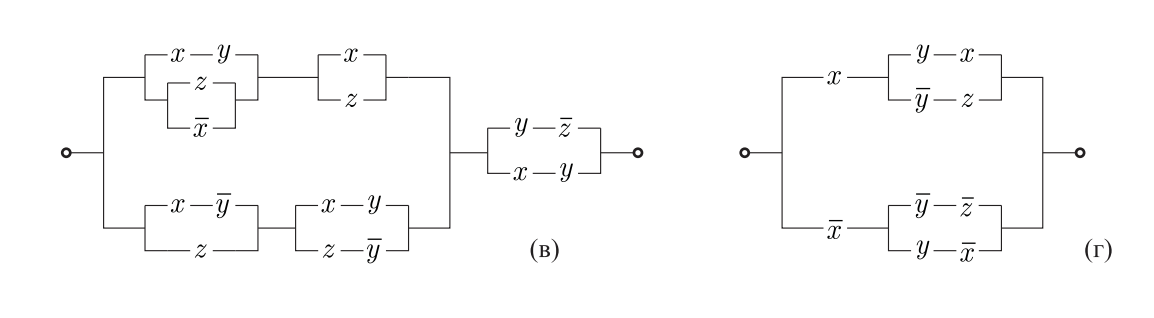
\includegraphics[width=140mm]{figure2}
			\end{center}
		\end{figure}
		
		\item Пабудуйце рэлейна-кантактныя схемы па зададзеных функцыях праводнасці і ўказанай колькасці кантактаў $h$:\\
		\ruText{Постройте релейно-контактные схемы по заданным функциям проводимости и указанному числу контактов $h$:}
		\begin{belarusianEnumerate}
			\item $(\overline{x \cdot \overline{y} \cdot z} \to (z \cdot t)) \vee
			(\overline{\overline{x} \vee y \vee \overline{z}}) \vee (\overline{z} \cdot t)$,\,\, $h \le 4$;
			
			\item $((x \vee y) \cdot (y \vee \overline{x \cdot z})) \to (\overline{\overline{y} \vee
				(x \cdot z) \vee \overline{x \vee z}})$,\,\, $h \le 8$;
			
			\item $((x \cdot y) \vee (y \cdot z)) \to (x \cdot z)$,\,\, $h \le 5$;
			
			\item $\overline{\overline{x \thicksim y} \cdot \overline{z}}$,\,\, $h \le 5$.
		\end{belarusianEnumerate}
	
		\bigskip
		
		\item Камітэт з трох чалавек вырашыў прымяніць электрычную схему для рэгістрацыі тайнага галасавання простай большасцю галасоў. Пабудуйце такую схему, пры выкарыстанні якой чалавек націскаў бы на кнопку, прычым у выпадку прыняцца рашэння загаралася б сігнальная лямпачка.\\
		\ruText{Комитет из трех человек решил применить электрическую схему для регистрации тайного голосования простым большинством голосов. Постройте такую схему, при использовании которой голосующий нажимал бы на кнопку, причем в случае принятия решения загоралась бы сигнальная лампочка.}
		
		\bigskip
		
		\item Катітэт складаецца з чатырох чалавек, адзін з якіх з'яўляецца старшынёй. Рашэнне выносіцца большасцю галасоў, прычым у выпадку роўнасці колькасці галасоў <<за>> і <<супраць>> вырашальным лічыцца голас старшыні. Пабудуйце такую схему, каб, галасуючы, кожны з чатырох чалавек націскаў бы на кнопку і ў выпадку прыняцца рашэння загаралася б сігнальная лямпачка. \\
		\ruText{Комитет состоит из четырех человек, один из которых является председателем. Решение выносится большинством голосов, причем в случае равенства числа голосов <<за>> и <<против>> решающим считается голос председателя. Постройте такую схему, чтобы, голосуя, каждый из четырех человек нажимал бы на кнопку и в случае принятия решения зажигалась бы сигнальная лампочка.}
		
		 \bigskip
		 
		 \item З кантактаў $x$, $y$, $z$, $t$ складзіце рэлейна-кантактную схему так, каб яна замкнулася (то-бок прапускала ток) тады і толькі тады, калі замкнуты якія-небудзь два з чатырох кантактаў $x$, $y$, $z$, $t$. \\
		 \ruText{Из контактов $x$, $y$, $z$, $t$ составьте релейно-контактную схему так, чтобы она замкнулась (т.~е. пропускала ток) тогда и только тогда, когда замкнуты какие-нибудь два из четырех контактов $x$, $y$, $z$, $t$.}
	\end{problemList}
\end{document}